\section{CNRS multiphysics benchmark} \label{sec:benchmark}

The \textit{CNRS benchmark} \citep{tiberga_results_2020} is a numerical
benchmark for multiphysics software dedicated to modeling \glspl{MSR}. It
consists of three Phases and eight Steps in total. Each
Step is a well-defined subproblem for systematically assessing the
capabilities of \gls{MSR} software and pinpointing sources of discrepancies
between software. Phase 0 consists three single-physics problems in fluid
dynamics, neutronics, and temperature, respectively. Phase 1 consists
of four coupled, steady-state problems. Lastly, Phase 2 consists of one
coupled, time-dependent problem.

\begin{figure}[htb!]
	\centering
	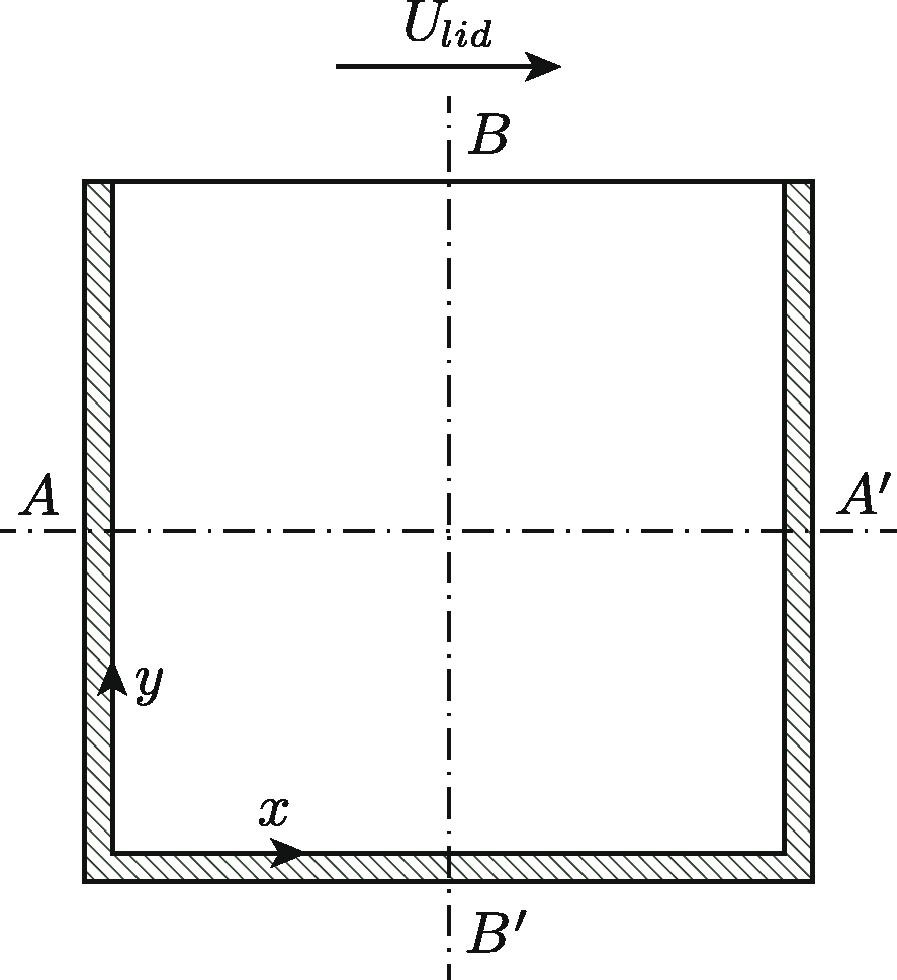
\includegraphics[width=.7\columnwidth]{geometry}
	\caption{2 m by 2 m domain of the \textit{CNRS benchmark}. $U_{lid}$
	represents the velocity along the top boundary. Various quantities are
	measured along the centerlines AA' and BB' for comparison. From
	\cite{tiberga_results_2020}.}
	\label{fig:geometry}
\end{figure}

As shown in Figure \ref{fig:geometry}, the domain geometry is a 2m by 2m square
cavity filled with LiF-BeF$_2$-UF$_4$ molten salt at an initial temperature of
900K \citep{tiberga_results_2020}.
Standard vacuum boundary conditions apply for neutron flux along all
boundaries, whereby outgoing neutrons are considered lost, while homogeneous
boundary conditions apply for delayed neutron precursors. No-slip boundary
conditions apply for velocity variables in the cavity, except along the top
boundary when the subproblem imposes forced flow in the form of lid-driven
cavity flow. For the temperature variable, all boundaries are insulated and we
simulate salt cooling with the following volumetric heat sink equation:
%
\begin{align}
    q'''(\vec{r}) &= \gamma \left(900 - T(\vec{r})\right), \label{eq:heat}
    \intertext{where}
    q''' &= \mbox{volumetric heat sink [W$\cdot$m$^{-3}$],}
    \nonumber \\
    \gamma &= \mbox{heat transfer coefficient [W$\cdot$m$^{-3}\cdot$K$^{-1}$],}
    \nonumber \\
    T(\vec{r}) &= \mbox{temperature at point $(\vec{r})$ [K].} \nonumber
\end{align}

\cite{tiberga_results_2020} used Serpent 2
\citep{leppanen_serpent_2014} with the JEFF-3.1 library
\citep{koning_jeff-31_2006} to generate multigroup neutronics data for the
LiF-BeF$_2$-UF$_4$ salt in the domain at 900K, condensed into six energy groups
and eight precursor groups. We direct readers to their paper for the
group constant data \citep{tiberga_results_2020}. In addition, the benchmark
prescribes the following equations to govern the temperature dependence in the
cross sections and the neutron diffusion coefficients:
%
\begin{align}
    \Sigma_i (T) &= \Sigma_i(T_{ref})
    \frac{\rho_{fuel}(T)}{\rho_{fuel}(T_{ref})}, \\
    D (T) &= D(T_{ref})
    \frac{\rho_{fuel}(T_{ref})}{\rho_{fuel}(T)},
    \intertext{where}
    \Sigma_i &= \mbox{relevant macroscopic cross section [cm${-1}$],}
    \nonumber \\
    D &= \mbox{neutron diffusion coefficient [cm$^2\cdot$s$^{-1}$],}   
    \nonumber \\
    \rho_{fuel} &= \mbox{density of the fuel salt [kg$\cdot$m$^{-3}$],}
    \nonumber \\
    T_{ref} &= \mbox{reference temperature} = 900\mbox{ K}. \nonumber
\end{align}

The benchmark also prescribes for incompressible Navier-Stokes flow and the
Boussinesq approximation for buoyancy when evaluating the salt flow in the
domain, but places no restrictions on the type of neutronics model.
The following subsections briefly detail each benchmark Step problem, namely
the input parameters and the measured observables from each Step.

\subsection{Phase 0: Single physics}

In this preliminary phase, the steady-state solutions of
individual physics are studied without any multiphysics coupling.

\subsubsection{Step 0.1: Velocity field}

This Step studies the steady-state incompressible flow distribution in the
domain from a lid-driven cavity flow by imposing a non-zero horizontal
velocity along the top boundary.

\subsubsection*{Input parameters}
\begin{itemize}
    \item $U_{lid} = 0.5$ m$\cdot$s$^{-1}$
\end{itemize}
%
\subsubsection*{Observables}
\begin{itemize}
    \item Velocity components, $u_x$ and $u_y$, along centerlines AA' and BB'
\end{itemize}

\subsubsection{Step 0.2: Neutronics}

This Step tests neutronics capabilities through a criticality eigenvalue
problem in a static, isothermal fuel configuration. The total power $P$ is
fixed to normalize the neutron fluxes.

\subsubsection*{Input parameters}
\begin{itemize}
    \item $U_{lid} = 0$ m$\cdot$s$^{-1}$
    \item $T = 900$ K
    \item $P = 1$ GW
\end{itemize}
%
\subsubsection*{Observables}
\begin{itemize}
    \item Fission rate density, $\sum^G_i \Sigma_{f,i} \phi_i(\vec{r})$, along
    AA'
    \item Reactivity, $\rho_{s_{0.2}}$
\end{itemize}

\subsubsection{Step 0.3: Temperature}

This Step studies the temperature distribution arising from a fixed velocity
field and a fission heat source distribution from Steps 0.1 and 0.2,
respectively.

\subsubsection*{Input parameters}
\begin{itemize}
    \item Fixed velocity field from Step 0.1
    \item Fixed fission heat source distribution from Step 0.2
    \item Heat transfer coefficient, $\gamma = 10^6$ W$\cdot$m$^{-3}\cdot$K$^{-1}$
\end{itemize}
%
\subsubsection*{Observables}
\begin{itemize}
    \item Temperature distribution, $T$, along AA' and BB'
\end{itemize}

\subsection{Phase 1: Steady-state coupling}

This phase builds towards a full multiphysics steady-state system by gradually
introducing coupling between various physics present in
a fast-spectrum molten salt system. All simulations are solved as steady-state
criticality eigenvalue problems.

\subsubsection{Step 1.1: Circulating fuel}

In this step, the delayed neutron precursors are allowed to drift under the
fixed velocity field from Step 0.1 while keeping the temperature $T$ fixed at
900 K. This criticality eigenvalue problem measures the reactivity loss from
the movement of precursors. The total power $P$ is fixed to normalize the
neutron fluxes.

\subsubsection*{Input parameters}
\begin{itemize}
    \item Fixed velocity field from Step 0.1
    \item $T = 900$ K
    \item $P = 1$ GW
\end{itemize}
%
\subsubsection*{Observables}
\begin{itemize}
    \item Delayed neutron source, $\sum_j \lambda_j C_j$, along AA' and BB'
    \item Reactivity change from Step 0.2, $\rho_{s_{1.1}} - \rho_{s_{0.2}}$
\end{itemize}

\subsubsection{Step 1.2: Power coupling}

In this step, the neutron fluxes and temperature are coupled to study the
interactions between neutronics and thermal-hydraulics under a fixed velocity
field. The effect of thermal feedback on the neutron cross sections and the
resulting change on the fission heat source distribution form a closed feedback
loop.

\subsubsection*{Input parameters}
\begin{itemize}
    \item Fixed velocity field from Step 0.1
    \item $P = 1$ GW
    \item Heat transfer coefficient, $\gamma = 10^6$ W$\cdot$m$^{-3}\cdot$K$^{-1}$
\end{itemize}
%
\subsubsection*{Observables}
\begin{itemize}
    \item Temperature distribution, $T$, along AA' and BB'
    \item Reactivity change from Step 1.1, $\rho_{s_{1.2}} - \rho_{s_{1.1}}$
    \item Change in fission rate density along AA' and BB' with respect to the
    corresponding solution from Step 0.2, $\sum^G_i \Sigma_{f,i} \phi_i(\vec{r}) - \left[\sum^G_i \Sigma_{f,i} \phi_i(\vec{r})\right]_{s_{0.2}}$
\end{itemize}

\subsubsection{Step 1.3: Buoyancy}

Building on the previous step, this step replaces the fixed velocity field with
buoyancy-driven flow arising from the temperature gradients. In turn, the flow
affects the neutron fluxes and temperature distributions through the advection
of \glspl{DNP} and temperature.

\subsubsection*{Input parameters}
\begin{itemize}
    \item $U_{lid} = 0$ m$\cdot$s$^{-1}$
    \item $P = 1$ GW
    \item Heat transfer coefficient, $\gamma = 10^6$ W$\cdot$m$^{-3}\cdot$K$^{-1}$
\end{itemize}
%
\subsubsection*{Observables}
\begin{itemize}
    \item Velocity components, $u_x$ and $u_y$, along centerlines AA' and BB'
    \item Temperature distribution, $T$, along AA' and BB'
    \item Delayed neutron source, $\sum_j \lambda_j C_j$, along AA' and BB'
    \item Reactivity change from Step 0.2, $\rho_{s_{1.3}} - \rho_{s_{0.2}}$
\end{itemize}

\subsubsection{Step 1.4: Full coupling}

This step reintroduces forced flow through the non-zero $U_{lid}$ boundary
condition. Thus, this problem most closely represents a molten salt system with
1) flow driven by an external force, 2) buoyancy flow effects, 3) \gls{DNP}
drift, and 4) thermal feedback effects on the neutronics. The steady-state
simulations are solved for a range of $U_{lid}$ and $P$ values given here.

\subsubsection*{Input parameters}
\begin{itemize}
    \item $U_{lid} \in [0, 0.1, 0.2, 0.3, 0.4, 0.5]$ m$\cdot$s$^{-1}$
    \item $P \in [0.2, 0.4, 0.6, 0.8, 1]$ GW
    \item Heat transfer coefficient, $\gamma = 10^6$ W$\cdot$m$^{-3}\cdot$K$^{-1}$
\end{itemize}
%
\subsubsection*{Observables}
\begin{itemize}
    \item Reactivity change from Step 0.2, $\rho_{s_{1.4}} - \rho_{s_{0.2}}$
\end{itemize}

\subsection{Phase 2: Time dependent coupling}

In this phase, the transient response of the fully coupled nonlinear system is
studied.

\subsubsection{Step 2.1: Forced convection transient}

Linear perturbation analyses are performed in this step by introducing periodic
perturbations to the heat transfer coefficient $\gamma$ and studying the gain
and phase shift of the response in the total power $P$. For the initial
conditions, the steady-state solution from Step 1.4 with
$U_{lid} = 0.5$ m$\cdot$s$^{-1}$ and $P = 1$ GW is used. This initial
configuration is made exactly critical by scaling the neutron source terms,
from fission and \gls{DNP} decay, by the inverse of the criticality eigenvalue
solution from Step 1.4.

$\gamma$ is uniformly perturbed according to small-amplitude sine waves given
as:
\begin{align}
    \gamma =& \gamma_0 \left[ 1 + 0.1\sin\left(2 \pi f \right) \right], \\
    \intertext{where}
    \gamma_0 =& 10^6 \mbox{ W$\cdot$m$^{-3}\cdot$K$^{-1}$}, \nonumber \\
    f \in& [0.0125, 0.025, 0.05, 0.1, 0.2, 0.4, 0.8]. \nonumber
\end{align}

\subsubsection*{Initial conditions}
\begin{itemize}
    \item Steady-state solution from Step 1.4 with
    $U_{lid} = 0.5$ m$\cdot$s$^{-1}$ and $P = 1$ GW
    \item Heat transfer coefficient, $\gamma = 10^6$ W$\cdot$m$^{-3}\cdot$K$^{-1}$
\end{itemize}
%
\subsubsection*{Observables}
\begin{itemize}
    \item Power gain $= \frac{\left(P_{max} - P_{avg}\right)/P_{avg}}{
    \left(\gamma_{max} - \gamma_{avg}\right)/\gamma_{avg}}$
    \item Power phase shift $=\theta_P - \theta_\gamma$
\end{itemize}
